% https://en.wikipedia.org/wiki/Capacitor#DC_circuits

\documentclass{article} %minimal is cool too

\usepackage{graphicx}
\usepackage[outdir=./]{epstopdf} % for including .esp

\usepackage{empheq} % for equation highlighting

\usepackage{amsmath}

\usepackage{hyperref}

\begin{document}

\title{Derivation of the Normal Vector to an Electric Potential Surface}
\author{Joe Iddon}
\date{March 20, 2020}
\maketitle

The electric potential field is three dimensional and scalar. A two dimensional electric potential field, concerned only with charges in the same XY-plane, can be visualised by a surface, $\textbf{S}$. The Z-dimension of the surface is equal to the electric potential at the corresponding XY-coordinate.

%https://en.wikipedia.org/wiki/Surface_(mathematics)#Graph_of_a_bivariate_function

The surface can be parametrised by a bivariate function $z = f(x,y)$. This function, $f(x,y)$, must calculate the electric potential at the point $(x,y)$ given the locations and charge of all known charges.

The electric potential at position $\vec{r}=(x,y)$ due to charge $i$ is given by

$$V = -k\frac{q_i}{|\vec{r}-\vec{r_i}|} = -k\frac{q_i}{\sqrt{(x-x_i)^2 + (y-y_i)^2}}$$

where the charge has location $\vec{r_i} = (x_i, y_i)$, and charge $q_i$.

Due to the principle of super position, the total electric potential can be calculated by summing over all charges.

\begin{equation}f(x,y) = -k\sum_{i}\frac{q_i}{\sqrt{(x-x_i)^2 + (y-y_i)^2}}\label{eqn:potential}\end{equation}

This describes $\textbf{S}$, allowing it to be easily plotted using computer software by iterating over a grid of $(x,y)$ locations and generating the height of the surface using this formula. The surface can then be triangulated and rendered. This can be seen in Figure~\ref{fig:no-shading}.

\begin{figure}
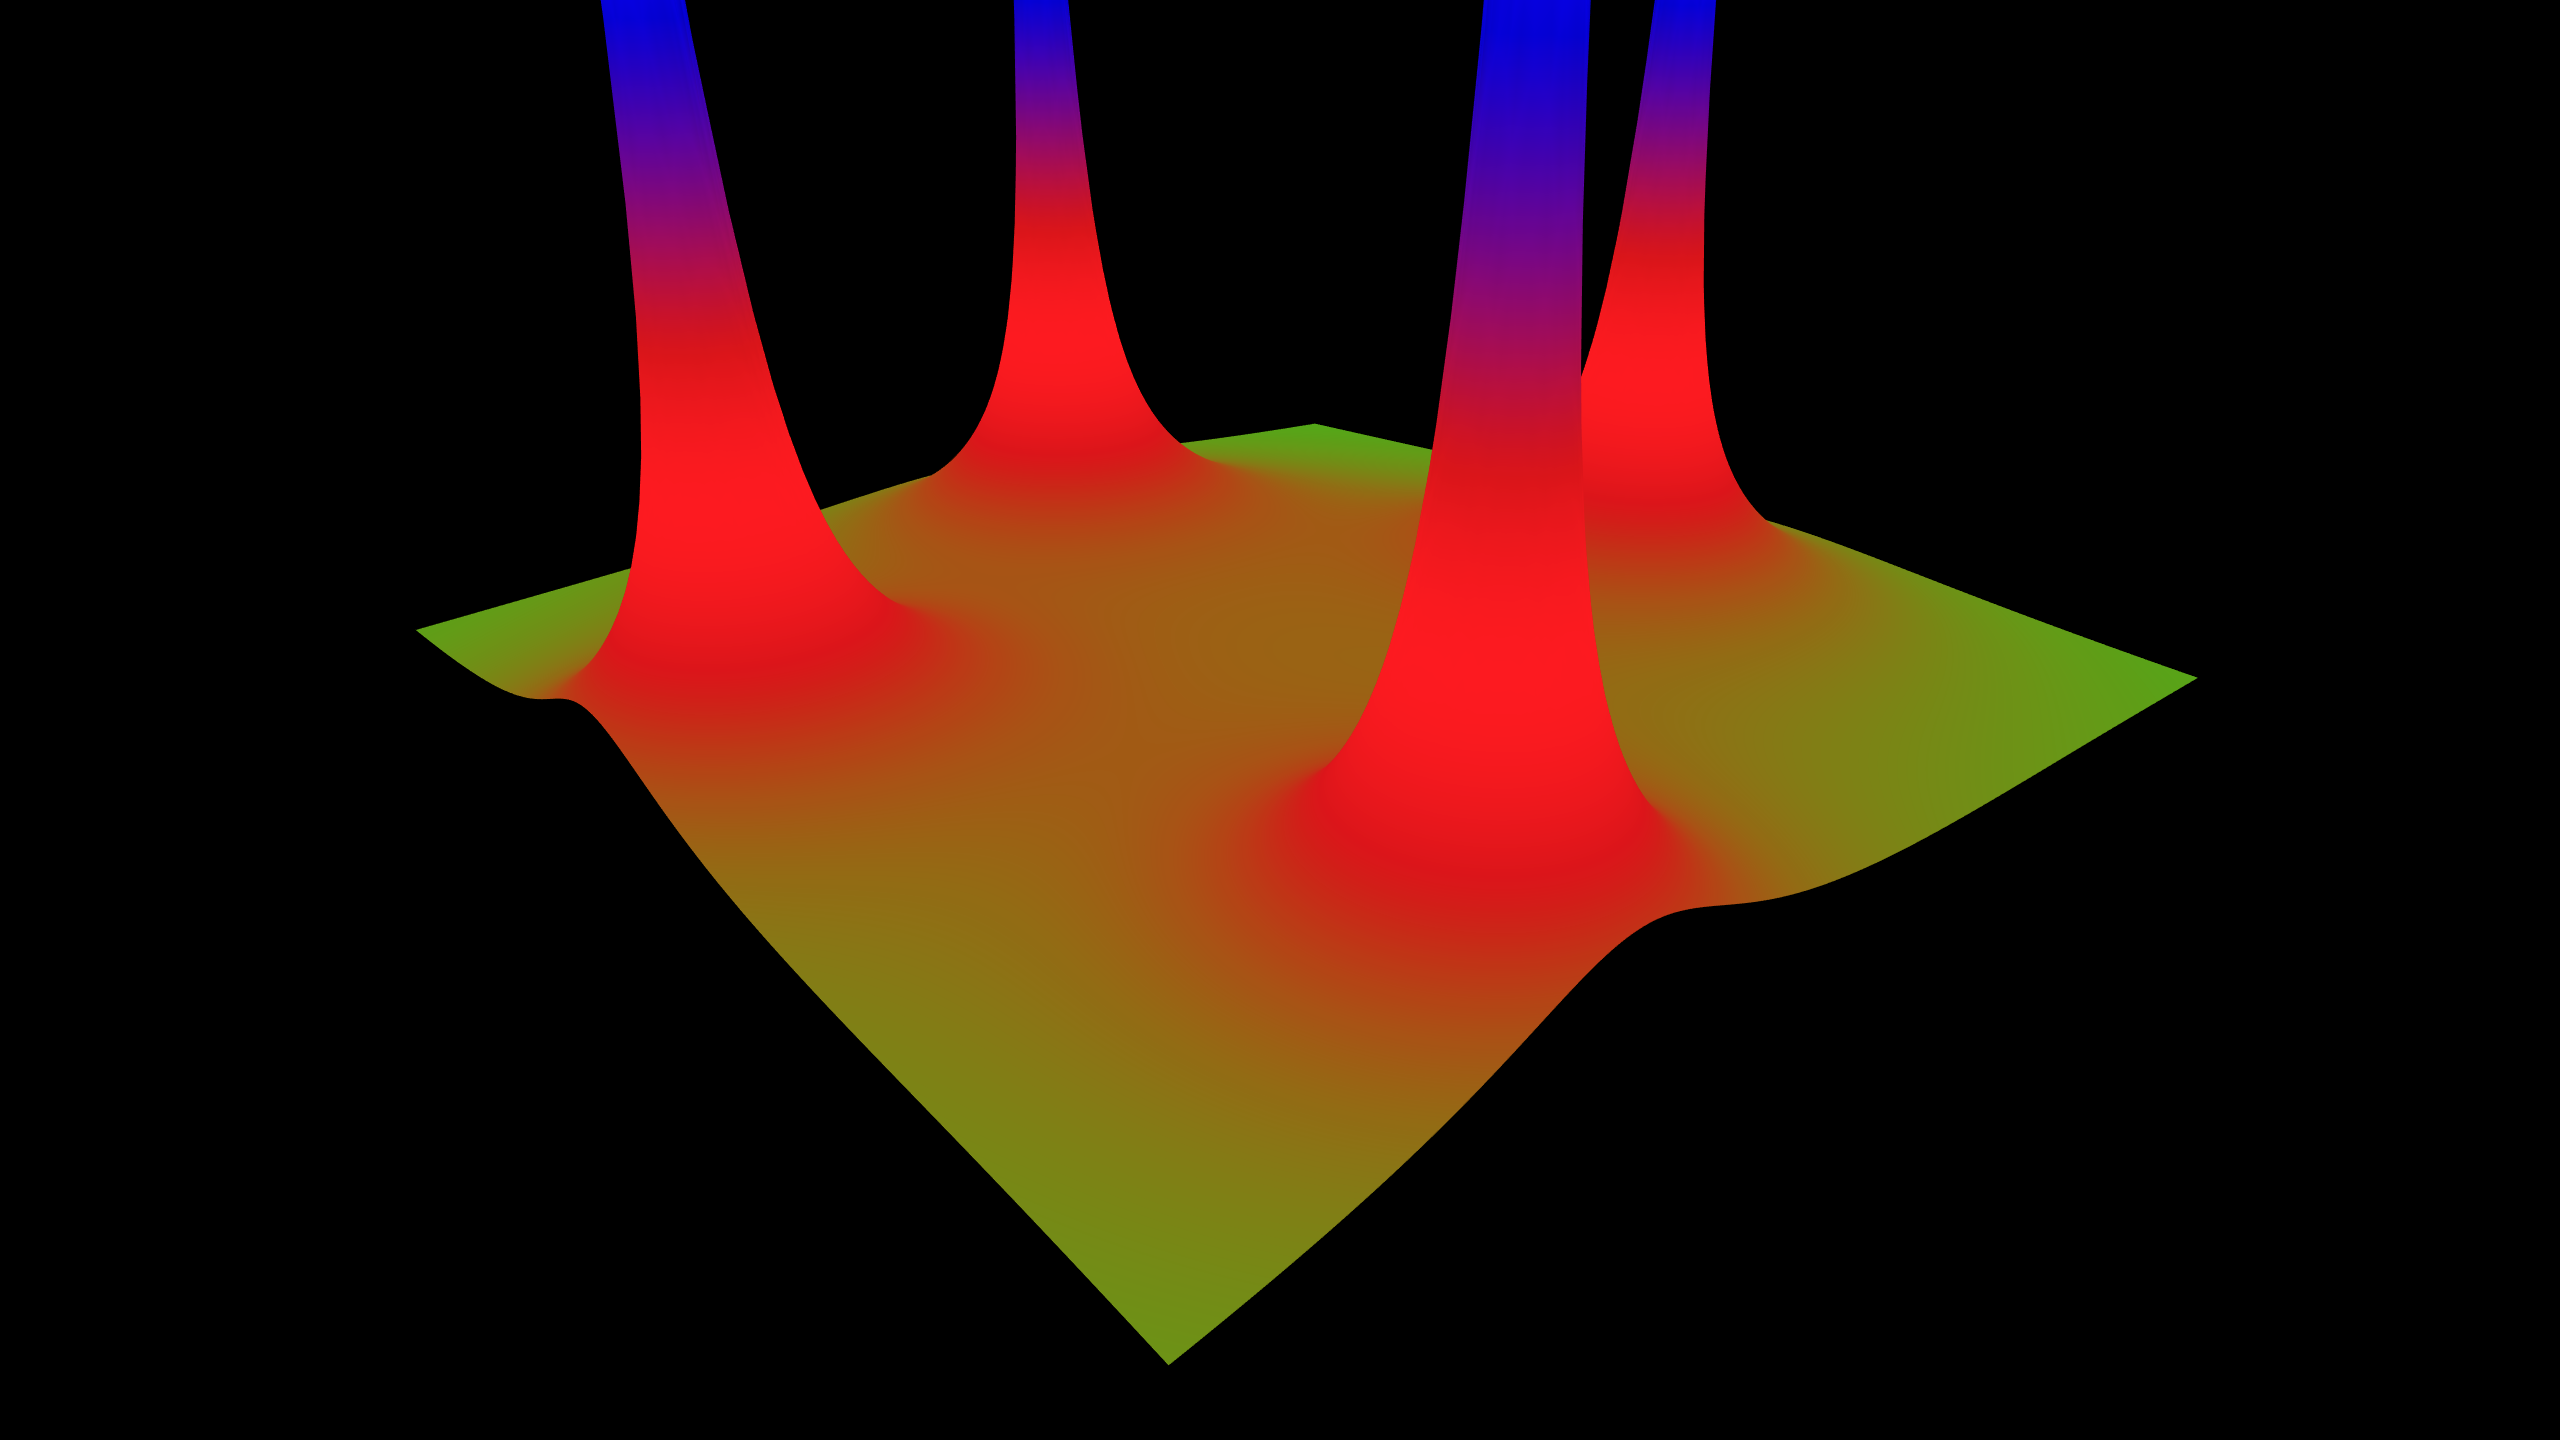
\includegraphics[width=\linewidth]{no_shading.png}
\caption{A visualisation of the electric potential without shading.}
\label{fig:no-shading}
\end{figure}

 This is a decent visualisation, but lacks distinction between peaks. To improve this lighting effects (shading) can be added.

 Rendering lighting is most simply done by multiplying the colour of each fragment by an intensity value. This intensity should represent how perpendicular the face is to the light source.

 The simplest way to calculate this intensity value is to take the dot product of the normal to the face with a light direction vector.

 The question is now, how can these normals be calculated. The most basic approach would be to take the three vertices of the surface and take the cross product of any two vectors between them. This would would work, however it is inefficient under the WebGL rendering method.

 The WebGL graphics library likes to work in terms of individual vertices in the vertex shader and, in general, each vertex is not aware of the other vertices it is connected to. This means the most standard approach would be to pre-calculate the normals for each face and pass these in alongside each vertex.

 However, this is inefficient as the code for calculating the vertices beforehand would not lie inside the vertex shader and could therefore not be run in parallel on the computers graphics processing unit.

 So a better solution to calculate the normal would be to use the surface equation, $f(x,y)$ directly. The normal to a surface can be calculated if the function of the surface is parametrised.

 The derivation for the normal of a surface is seen below.

 Consider Figure~\ref{fig:diagram}, the axis have been centred on the current position on the surface $\textbf{S}$ (highlighted in red) where we want to calculate the normal (labelled as as $\vec{n}$).

 \begin{figure}
    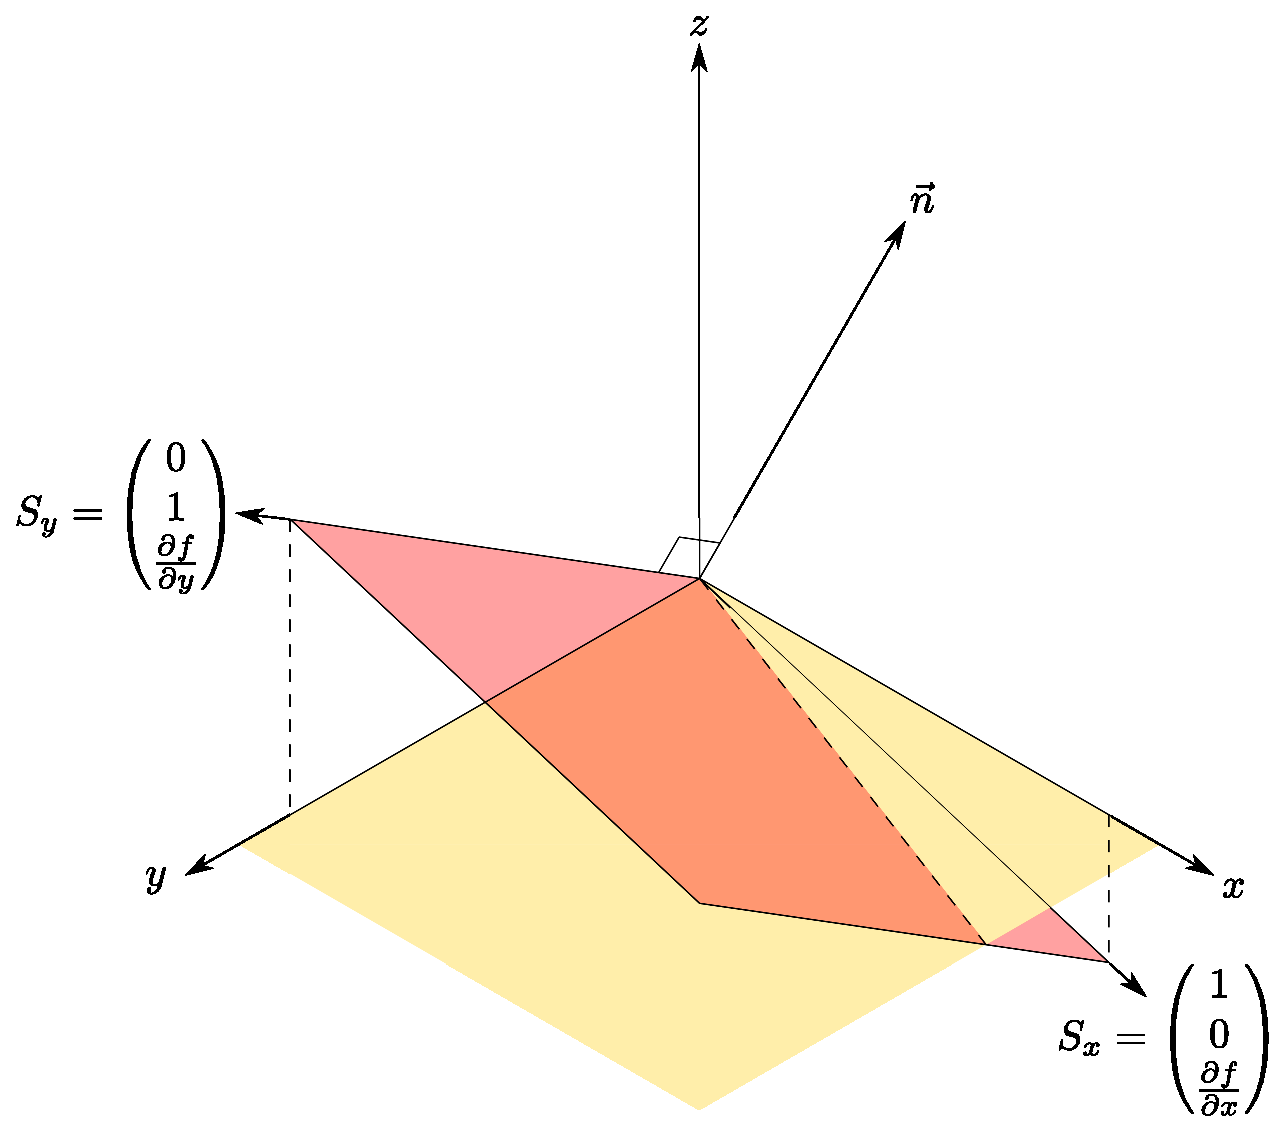
\includegraphics[width=\linewidth]{diagram.eps}
    \caption{A section of the electric potential surface $S$. The axis are centred at a point on the surface where we want to calculate the normal. Two vectors are defined, $S_x$ and $S_y$ that lie along the surface in the X- and Y-directions. The cross product of these is equal to the normal of the surface, $\vec{n}$.}
    \label{fig:diagram}
    \end{figure}

 Let us define two vectors that both lie along the surface as well either the XZ-plane or YZ-plane as $S_x$ and $S_y$, respectively. Both these vectors will have the length along their bases (the components along the x-axis and y-axis, respectively) set as one (See diagram).

 The gradient of the surface in the X- and Y-directions are given by $\frac{\partial f}{\partial x}$ and $\frac{\partial f}{\partial y}$, respectively. Since the bases of the two vectors have been defined to have length one, their heights are therefore equal to these partial derivatives.

 This gives the two vectors as

$$
S_x = \begin{pmatrix}1 \\ 0 \\ \frac{\partial f}{\partial x}\end{pmatrix}\textrm{ and }
S_y = \begin{pmatrix}0 \\ 1 \\ \frac{\partial f}{\partial y}\end{pmatrix}.
$$

 Now the normal vector can be calculated directly at this point as as the cross product of these two vectors.

$$\vec{n} = S_x \times S_y = \begin{vmatrix*}[r]
\hat{i} & \hat{j} & \hat{k} \\
1 & 0 & \frac{\partial f}{\partial x} \\
0 & 1 & \frac{\partial f}{\partial y}
\end{vmatrix*} =
\begin{pmatrix}-\frac{\partial f}{\partial x} \\ -\frac{\partial f}{\partial y} \\ 1\end{pmatrix}
$$

This result makes intuitive sense when considering the diagram: the vector should have a positive Z-component and should point in the opposite direction to the gradient in each dimension (note the gradient in the X-direction is negative in the diagram so the normal vector has a positive X-component).

Finally, to be of use in lighting calculations, this vector should then be normalised.

\begin{equation}\hat{n} = \frac{\vec{n}}{|\vec{n}|} =
\frac{1}{\sqrt{
    \frac{\partial f}{\partial x}^2 +
    \frac{\partial f}{\partial x}^2 +
    1
}}
\begin{pmatrix}-\frac{\partial f}{\partial x} \\ -\frac{\partial f}{\partial y} \\ 1\end{pmatrix}
\label{eqn:normal}\end{equation}

This formula is general, but we are interested in the specific case of the electric potential field defined by Equation~\ref{eqn:potential}. To be able to combine this equation with \ref{eqn:normal}, we must calculate the partial derivatives which can then be plugged straight in to this formula.

The sum can be drawn outside the derivative, and then the function can be differentiated treating everything as constant which is not what we are differentiating with respect to.

This gives that

\begin{align*}
\frac{\partial f}{\partial x} = &\frac{\partial}{\partial x}(-k\sum_{i}\frac{q_i}{\sqrt{(x-x_i)^2 + (y-y_i)^2}})\\
=&-k\sum_{i}q_i\frac{\partial}{\partial x}((x-x_i)^2 + (y-y_i)^2)^{-\frac{1}{2}} \\
=&-k\sum_{i}q_i \cdot -\frac{1}{2} ((x-x_i)^2 + (y-y_i)^2)^{-\frac{3}{2}} \cdot 2(x-x_i) \\
=&k\sum_{i}\frac{q_i(x-x_i)}{(\sqrt{(x-x_i)^2 + (y-y_i)^2})^3} \\
=&k\sum_{i}\frac{q_i(x-x_i)}{|\vec{r}-\vec{r_i}|^3}
\end{align*}

Similarly,

$$\frac{\partial f}{\partial y} = k\sum_{i}\frac{q_i(y-y_i)}{|\vec{r}-\vec{r_i}|^3}$$

Implementing this calculation in the WebGL Shader Language (GLSL), gives the much nicer result found in Figure~\ref{fig:shading}.

\begin{figure}
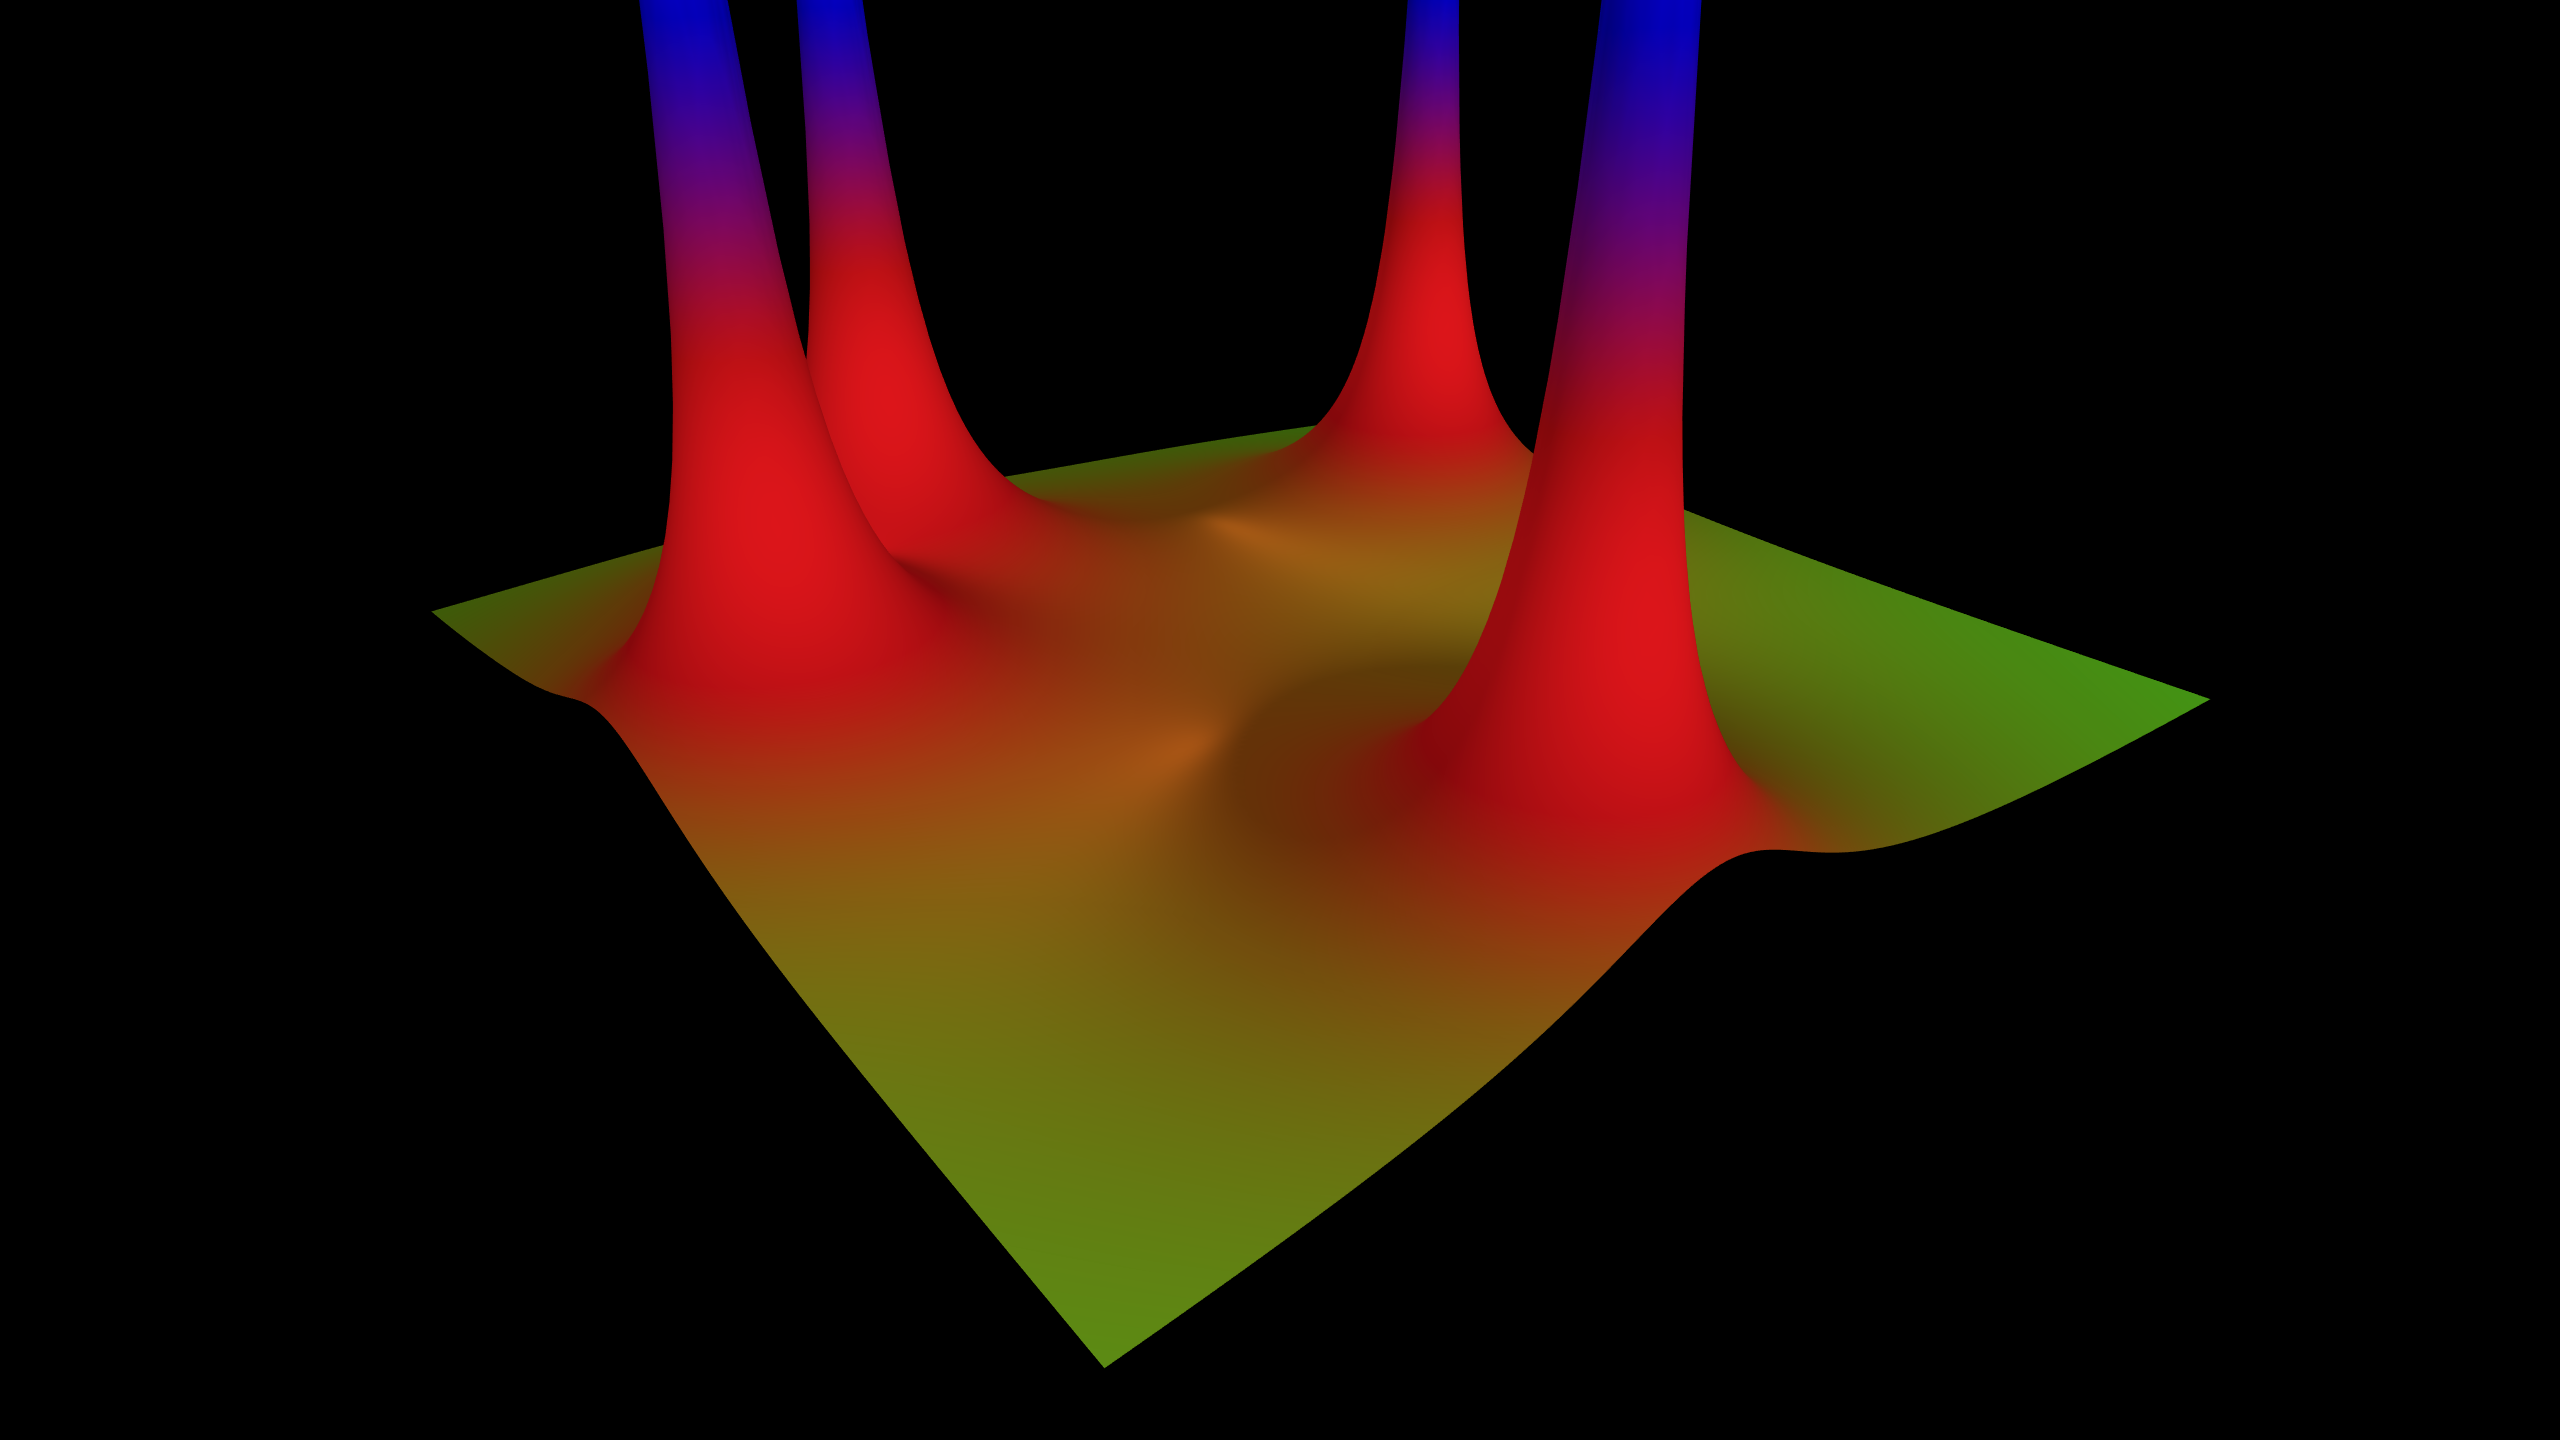
\includegraphics[width=\linewidth]{shading.png}
\caption{A visualisation of the electric potential with shading.}
\label{fig:shading}
\end{figure}

\vfill

The final result can be found at:

\begin{center}
\url{https://joeiddon.github.io/fields/electric_potential}
\end{center}

Controls: use the left mouse button to place charges, click and hold the right mouse button to pan.

\end{document}